\chapter{Прочные конструкции}
{\bfseries Анонс:}\\\\
Принципы построения прочных конструкций: ребра жесткости, шарнирные соединения, принципы треугольников. Задача на прочную конструкцию. Самонатягивающиеся конструкции.\\\\
{\bfseries Цели:}
\begin{itemize}
	\item{}{\bfseries Обучающие:} Знакомство с основными принципами проектирования жестких конструкций. Закрепление принципа «диагональных ребер».
	\item{}{\bfseries Развивающая:} Развитие творческих навыков, пространственного воображения, любознательности учащихся.\\
\end{itemize}	
{\bfseries Ход занятия:}\\\\
\begin{tabular}[h!]{lll}
	{\hyperlink{lesson19x1}{1. Организационный момент}}&{Презентация}&{(5 мин)}\\
	{\hyperlink{lesson19x2}{2. Плоские балочные конструкции}}&{Презентация + Практика}&{(20 мин)}\\
	{\hyperlink{lesson19x3}{3. Объемные балочные конструкции}}&{Презентация + Практика}&{(20 мин)}\\
	{\hyperlink{lesson19x4}{4. Деформируемые конструкции}}&{Презентация + Практика}&{(25 мин)}\\
	{\hyperlink{lesson19x5}{5. Соединения шестеренок}}&{Презентация + Практика}&{(15 мин)}\\
	{\hyperlink{lesson19x6}{6. «Прочная тележка»}}&{Практика}&{(35 мин)}\\
	{\hyperlink{lesson19x7}{7. Самонапряженные конструкции*}}&{Презентация + Практика}&{(20 мин)}\\
\end{tabular}\\\\

{\hypertarget{lesson19x1}{\blackBlueText{I. Организационный момент}}}\\\\	

Практически в течение всего этого занятия учащиеся работают параллельно с учителем. Учитель объясняет новый материал и демонстрирует сборку разнообразных конструкций из деталей набора, удобно делать это перед камерой и транслировать изображение на большой экран. Учащиеся повторяют за ним и время от времени получают небольшие задания для самостоятельного творчества.

Для работы по разделам 2--6 достаточно стандартного набора деталей. Раздел 7 является дополнительным, для работы в нем понадобятся нитки и карандаши.\\\\

\greenText{Куб в 3 разделе?}\\\\

{\hypertarget{lesson19x2}{\blackBlueText{II. Плоские балочные конструкции}}}\\\\

Проектирование и конструирование различных сооружений, машин и механизмов основано на жестких конструкциях. Нехорошо, когда скамейка на улице шатается, дом подкашивается или деревянный мост прогибается под тяжестью груженого автомобиля. В быту понятие «жесткий» часто смешивается с понятием «прочный», хотя на практике это не всегда верно. От собираемых роботов также требуется устойчивость конструкции. К тому же во многих соревновательных задачах роботу предстоит сталкиваться с другими роботами, возможно, падать и прочими способами взаимодействовать с твердыми материальными объектами. Для успешного выполнения поставленных задач конструкция робота должна быть жесткой, никакие ее части не должны иметь возможность бесконтрольно перемещаться относительно других. 

Основной тип деталей, используемых в конструкторе Lego Mindstorms~--- балки. Поэтому наибольшее внимание будет уделено именно балочным конструкциям. По мнению автора, разумно выделить два главных принципа: назовем их принцип А и принцип Б.

Принцип А~--- это первое приближение, первый шаг при планировании сборки. Представим, что все наши балки~--- это абсолютно жесткие стержни. Жесткие~--- значит не имеют возможности гнуться и математически представимы прямыми отрезками. В конструкторе Lego Mindstorms балки соединяются штифтами. При этом у двух соединенных балок остается возможность вращаться друг относительно друга. Соединение штифтом~--- частный случай шарнирного соединения. Поэтому принцип, который мы обозначили буквой А является принципом жестких балок и шарнирных соединений между ними. Рассмотрим простые примеры возможных конструкций, вначале плоских.

Соберем из балок параллелограмм.\\\\

\greenText{Рис}\\\\

Легко заметить, что если попытаться немного пошевелить конструкцию и сдвинуть верхнюю горизонтальную балку относительно нижней, то конструкция легко меняет форму. 

{\slshape Вопрос учащимся: Как можно с этим бороться?
	
	На размышления дается 3--5 минут.}	

Поставим диагональную балку, соединив верхний левый угол с нижним правым:\\\\

\greenText{Рис}\\\\

В плоскости наша конструкция теперь не может двигаться. Заметим, что добавление диагонали разбило параллелограмм на два треугольника. Оказывается, что треугольник в плоскости (на самом деле и в пространстве) всегда является жесткой конструкцией. В самом деле, если мы возьмем одну вершину треугольника и попытаемся ее переместить, то все остальные вершины обязательно тоже переместятся. Треугольник перемещается как одно целое, без изменения относительного расположения своих сторон.

\begin{figure}[h!]
	\begin{center}
		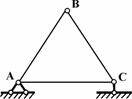
\includegraphics[width=0.3\linewidth]{chapters/chapter19/images/1}
		\caption{}
		\label{ris:image19x1}
	\end{center}
\end{figure}

{\hypertarget{lesson19x3}{\blackBlueText{III.  Объемные балочные конструкции}}}\\\\

Следующий небольшой шаг, который нужно сделать~--- научиться создавать трехмерные жесткие конструкции. Рассмотрим пример куба.

\greenText{Как собрать куб из лего} или из чего-то другого?

Будем рассматривать возможные деформации сдвига. Как видно из рисунка, существует 3 возможных способа деформировать куб таким образом. Заметим, что число возможностей совпадает с числом осей координат и с размерностью нашего геометрического пространства. Если мы добавим диагональ в квадрате одной из граней куба, то мы зафиксируем таким образом одну из внутренних степеней свободы. То есть куб не сможет деформироваться вокруг одной из трех координатных осей (см. рисунок). Если мы добавим диагональ у противоположной, параллельной грани, то, учитывая жесткость всех ребер, это не придаст конструкции дополнительной стабильности. Попробуем теперь добавить диагональ в перпендикулярной грани. Это приведет к запрету деформации сдвига во втором направлении – вокруг второй оси (см. рисунок). Останется только возможность искривлять куб вокруг третьей оси. Исправить это можно, добавив диагональ в грани, перпендикулярной первым двум. Таким образом, для того, чтобы куб (состоящий из жестких ребер и шарнирных соединений) стал жестким, необходимо добавить диагонали (треугольники) в трех взаимно перпендикулярных плоскостях.\\\\

\greenText{Рисунки куба, иллюстрирующие все вышесказанное}\\\\

Резюмируем вышесказанное. Принцип жестких стержней и шарнирных соединений заключается в требовании неподвижности одних узлов конструкции относительно других при всевозможных попытках деформации. Добиться этого можно добавляя треугольники (или диагонали в четырехугольниках). При этом минимальный набор треугольных элементов~--- три, во взаимно перпендикулярных плоскостях.

{\slshape Вопрос учащимся: Какие бытовые примеры жестких конструкций из треугольников вы можете привести?}

Если мы оглянемся вокруг, то в конструкции окружающих нас предметов сплошь и рядом встречаются треугольники: деревенские калитки и металлические ограды, опоры светофоров, дорожных знаков и рекламных щитов, конструкции железнодорожных мостов и опор линий электропередач. Использовать треугольники в строительстве начали очень давно: один из интересных примеров~--- Фахверк~--- дома, которые повсеместно являются туристическими достопримечательностями. При строительстве вначале сооружался каркас, обязательно включающий в себя треугольные элементы. Затем пространство между балками заполнялось травой, глиной, известью, цементным раствором, в зависимости от периода, в который дом строился.\\\\

\greenText{Фотография фахверка}\\\\
\clearpage
\begin{figure}[h!]
	\begin{center}
		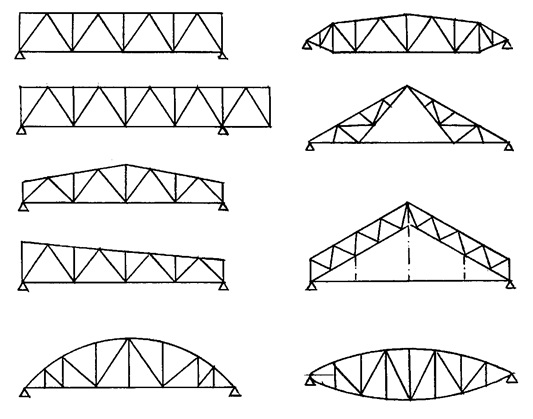
\includegraphics[width=1\linewidth]{chapters/chapter19/images/2}
		\caption{}
		\label{ris:image19x2}
	\end{center}
\end{figure}

Применительно к конструированию с использованием Lego Mindstorms следует отметить тот факт, что некоторые детали уже представляют собой аналог треугольника при нужном количестве соединительных штифтов. Примеры таких деталей~--- уголки, Т-образная балка, сам блок NXT и другие.\\\\

\greenText{Фотографии таких деталей с нарисованным треугольником}\\\\

Использование таких деталей несколько упрощает задачу, ведь проще придумать, как соединить две перпендикулярные балки уголком, чем думать, как добавить в такое соединение диагональ, см. \greenText{рисунок}.\\\\

\greenText{Иллюстрация простоты соединения уголком, проблема добавления диагонали (детали не попадают в нужные плоскости)}\\\\

{\hypertarget{lesson19x4}{\blackBlueText{IV. Деформируемые конструкции}}}\\\\

Принцип Б~--- второе приближение, более близкое к реальности. Предположим, что балки теперь имеют возможность изгибаться. Деформация самих балок, стержней конструкции, вносит дополнительные внутренние степени свободы в конструкцию. Трудно предложить универсальные алгоритмы в таких случаях. В каждой ситуации необходимо продумывать, что произойдет с конструкцией при возможном изгибе при известных нагрузках на конструкцию. Искусство инженера в таких случаях проявляется в добавлении таких элементов, которые компенсируют возможные напряжения и не позволят элементам деформироваться. При анализе конструкции важно понимать, что чем длиннее балка, тем больше ее деформация изменит геометрию всей конструкции. То есть первым делом внимание следует уделять укреплению длинных элементов конструкции. Приведем простой плоский пример, иллюстрирующий вышесказанное. 

Н-образная конструкция, оба соединения вертикальных и горизонтальной балки используют уголки (аналог треугольников). Но при приложении вертикальной силы, направленной вниз, нижние части вертикальных балок начнут «разъезжаться», а горизонтальная балка прогибаться. Исправить ситуацию можно добавив горизонтальную балку, соединяющую два верхних конца вертикальных балок.

Итак, при проектировании любой, даже самой простой конструкции рекомендуется в обязательном порядке следовать двум принципам. Прежде всего~--- принципу жестких стержней и шарнирных соединений (Принцип А). Затем~--- исследовать конструкцию на возможные деформации при прикладываемых нагрузках и усилить слабые узлы (Принцип Б). Кроме этого, нужно помнить, что умелый конструктор~--- это тот, который способен реализовать оба принципа, используя минимальное количество деталей. Нагромождение деталей в большинстве случаев только усложняет конструкцию, далеко не всегда решая проблемы ее жесткости. Поэтому автор настоятельно рекомендует вначале продумать свою модель, возможно, нарисовать ее, и лишь затем приступать к сборке.\\\\

{\hypertarget{lesson19x5}{\blackBlueText{V. Соединения шестеренок}}}\\\\

В данной главе отдельно следует рассмотреть принципы и особенности шестереночных соединений. Самым слабым и легко деформируемым элементов в такой конструкции является ось. Она гораздо тоньше балок и поэтому легко гнется. К возможным изгибам осей нужно относиться очень внимательно. Представим, что на двух осях, продетых через балку, закреплены зацепляющиеся друг за друга  шестеренки, находящиеся с одной стороны балки. Если одной рукой удерживать одну из осей, а другой попытаться прокрутить вторую, то при некотором усилии шестеренки начнут проскакивать. Зубчатое соединение перестанет работать. Почему это происходит? Дело в том, что при таком усилии оси деформируются, и расстояние между центрами шестеренок увеличивается. Чтобы избежать таких ситуаций, можно установить балки с обеих сторон от шестеренок (см.\greenText{ рисунок}). В такой ситуации шестеренки могут проскакивать при довольно больших усилиях, которые, во-первых, редко возникают, а во-вторых, способны привести к поломке деталей, поэтому недопустимы. Итак, еще одно правило в добавок к принципам А и Б~--- требование к наличию балок с обеих сторон он шестеренок, формирующих зубчатое соединение. При этом естественно важно, чтобы оси, на которых закреплены шестеренки были продеты через обе балки.\\\\

{\hypertarget{lesson19x6}{\blackBlueText{VI. «Прочная тележка»}}}\\\\

Как мы помним, на втором занятии ребята строили самый длинный мост. И более прочная, более длинная устойчивая конструкция получалась у тех, кто использовал треугольники для жесткого закрепления балок друг относительно друга. Сегодняшнее задание требует осознанного применения всеми принципов А и Б, а также правила сборки зубчатых соединений. 

Задание~--- трехколесная тележка с максимально возможным передаточным соотношением на скорость (определяется доступным набором шестеренок). В задаче необходимо использовать колеса большого диаметра и как минимум 2 ступени зубчатой передачи. По сути, эта та «самая быстрая тележка», которую дети строили в Занятии 9. Однако, в рамках обновленной задачи, во-первых, необходимо применить правило сборки зубчатых соединений. В передаточных соединениях на скорость на оси мотора возникают существенные усилия, поэтому, если правилу не следовать, шестеренка на оси мотора обязательно будет проскакивать. Кроме этого, наличие нескольких передаточных соотношений делает конструкцию трехколесной тележки шире стандартной. В совокупности с использованием колес большого диаметра это создает проблемы жесткости конструкции: центр начинает проседать вниз, ведущие колеса заваливаться внутрь. Задача~--- справиться со всеми трудностями.

Главные мысли, которые должны найти отражение в детских конструкциях~--- больше треугольников, ставить стяжки, тестировать на изгибы и смещения готовые модели.\\\\

{\hypertarget{lesson19x6}{\blackBlueText{VII. Самонапряженные конструкции}}}\\\\

Дополнительно можно затронуть интереснейший вопрос самонапряженных конструкций.
Задача: Имеется  3 карандаша и нитки. Как из них собрать жесткую объемную конструкцию, которая будет сохранять свою форму без внешней помощи и даже способна выдержать падение с небольшой высоты? При этом требуется, чтобы стержни не соприкасались (ни непосредственно, ни «через нитки»).

Принцип тот же, что помогает при укреплении высоких мачт, антенн, труб,~--- использовать растяжки. Кто хоть раз видел такие конструкции, вспомнит, что обычно от них отходят в разные стороны три или четыре сильно натянутых троса, которые позволяют строениям не падать даже при очень сильном ветре. У нас в роли мачт выступят стержни, а в роли растяжек~--- нитки. Но за что их закрепить? Поскольку по условию ничего другого использовать нельзя, то придется закреплять за другие стержни. В итоге должно получиться, что от каждого конца каждого из трех стержней растяжки идут к концам двух других, которые должны перекрещиваться между собой.

\begin{figure}[h!]
	\begin{center}
		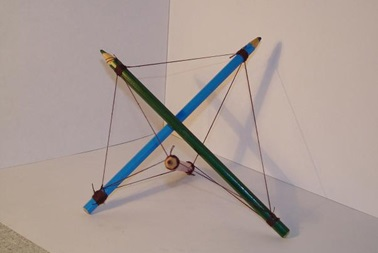
\includegraphics[width=1\linewidth]{chapters/chapter19/images/3}
		\caption{}
		\label{ris:image19x3}
	\end{center}
\end{figure}	

Правильный баланс натяжений-сжатий позволяет несущему скелету конструкции быть прочным и вмещать большой полезный объем. При этом он состоит из стандартных деталей, поэтому прост в производстве. Часто на фестивалях или других крупных мероприятиях, проходящих под открытым небом, можно видеть тенты и павильоны, в основе структуры которых заложен принцип самонапряжения.\\\\
\clearpage
Вот несколько сооружений, построенных по этому принципу:

\begin{itemize}
	\item Музей «Биосфера» (см. \href{http://en.wikipedia.org/wiki/Montreal_Biosph\%C3\%A8re}{\whiteBlueText{\underline{Biosphere}}}) в Монреале (Канада), спроектированный Фуллером. Первоначально это был павильон США на всемирной выставке 1967 года (\href{http://en.wikipedia.org/wiki/Expo_67}{\whiteBlueText{\underline{Expo 67}}}).
	
	\begin{figure}[h!]
		\begin{center}
			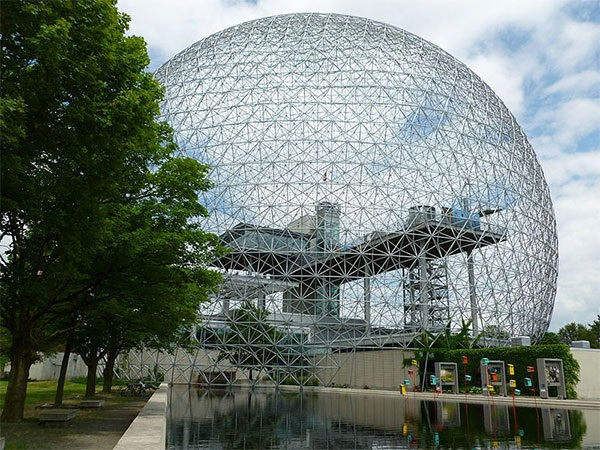
\includegraphics[width=0.84\linewidth]{chapters/chapter19/images/4}
			\caption{Музей «Биосфера» в Монреале (Канада)}
			\label{ris:image19x4}
		\end{center}
	\end{figure}
	
	\item Пешеходный мост Курилпа (см. \href{http://en.wikipedia.org/wiki/Kurilpa_Bridge}{\whiteBlueText{\underline{Kurilpa\_Bridge}}}) в Брисбене (Австралия). Это крупнейший мост, построенный по принципу тенсегрити.
	
	\begin{figure}[h!]
		\begin{center}
			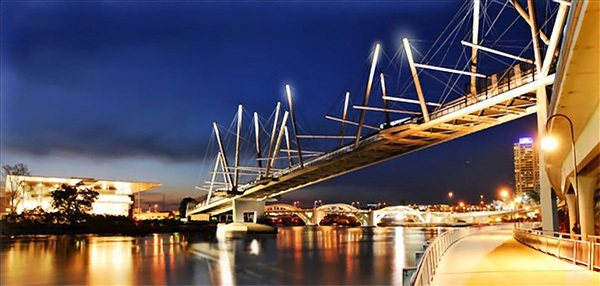
\includegraphics[width=0.84\linewidth]{chapters/chapter19/images/5}
			\caption{Пешеходный мост Курилпа в Брисбене (Австралия)}
			\label{ris:image19x5}
		\end{center}
	\end{figure}	
	\clearpage
	\item Башня «Игла» (см. \href{http://en.wikipedia.org/wiki/Needle_Tower}{\whiteBlueText{\underline{Needle Tower}}}), расположена возле музея Хиршхорна в Вашингтоне (США). Это сооружение высотой 18 метров было спроектировано учеником Фуллера К. Снельсоном в 1968 году.
	
	\begin{figure}[h!]
		\begin{center}
			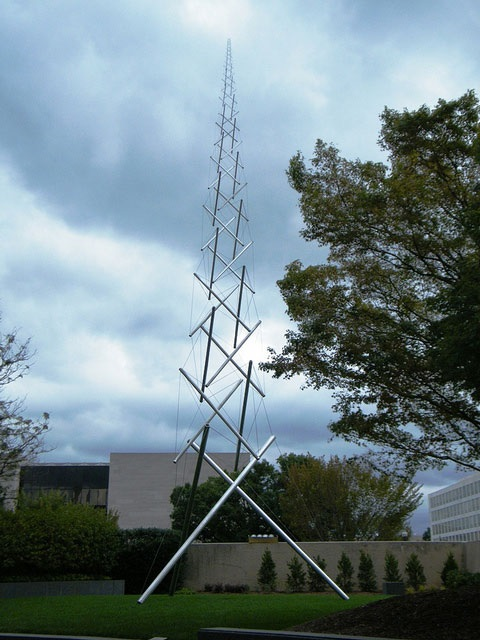
\includegraphics[width=0.97\linewidth]{chapters/chapter19/images/6}
			\caption{Башня «Игла», расположенная возле музея Хиршхорна в Вашингтоне (США)}
			\label{ris:image19x6}
		\end{center}
	\end{figure}	
\end{itemize}